\documentclass[border=6pt]{standalone}
\usepackage{tikz}
\begin{document}
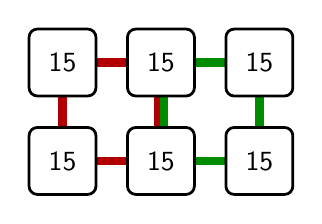
\begin{tikzpicture}[font=\sffamily,
    tile/.style={draw, rounded corners=3pt, fill=white, minimum size=0.85cm,
                 line width=1pt, inner sep=0pt},
    loopA/.style={line width=3pt, draw=red!70!black},
    loopB/.style={line width=3pt, draw=green!55!black}]
  \def\s{1.25}
  % first test case of example 1: full 2x3 grid, two loops
  \draw[loopA] (1*\s,-1*\s) -- (2*\s,-1*\s);
  \draw[loopA] (1*\s,-1*\s) -- (1*\s,-2*\s);
  \draw[loopA] (1*\s,-2*\s) -- (2*\s,-2*\s);
  \draw[loopB] (2*\s,-1*\s) -- (3*\s,-1*\s);
  \draw[loopB] (3*\s,-1*\s) -- (3*\s,-2*\s);
  \draw[loopB] (2*\s,-2*\s) -- (3*\s,-2*\s);
  \draw[loopA] (2*\s-0.035,-1*\s) -- (2*\s-0.035,-2*\s);
  \draw[loopB] (2*\s+0.035,-1*\s) -- (2*\s+0.035,-2*\s);
  \foreach \c/\r in {1/1, 2/1, 3/1, 1/2, 2/2, 3/2}
    \node[tile] at (\c*\s,-\r*\s) {15};
\end{tikzpicture}
\end{document}
